\subsection{Assessing gradience}

\subsubsection{Response distributions}

This is shown in Figure \ref{density}.

\begin{figure}
\centering
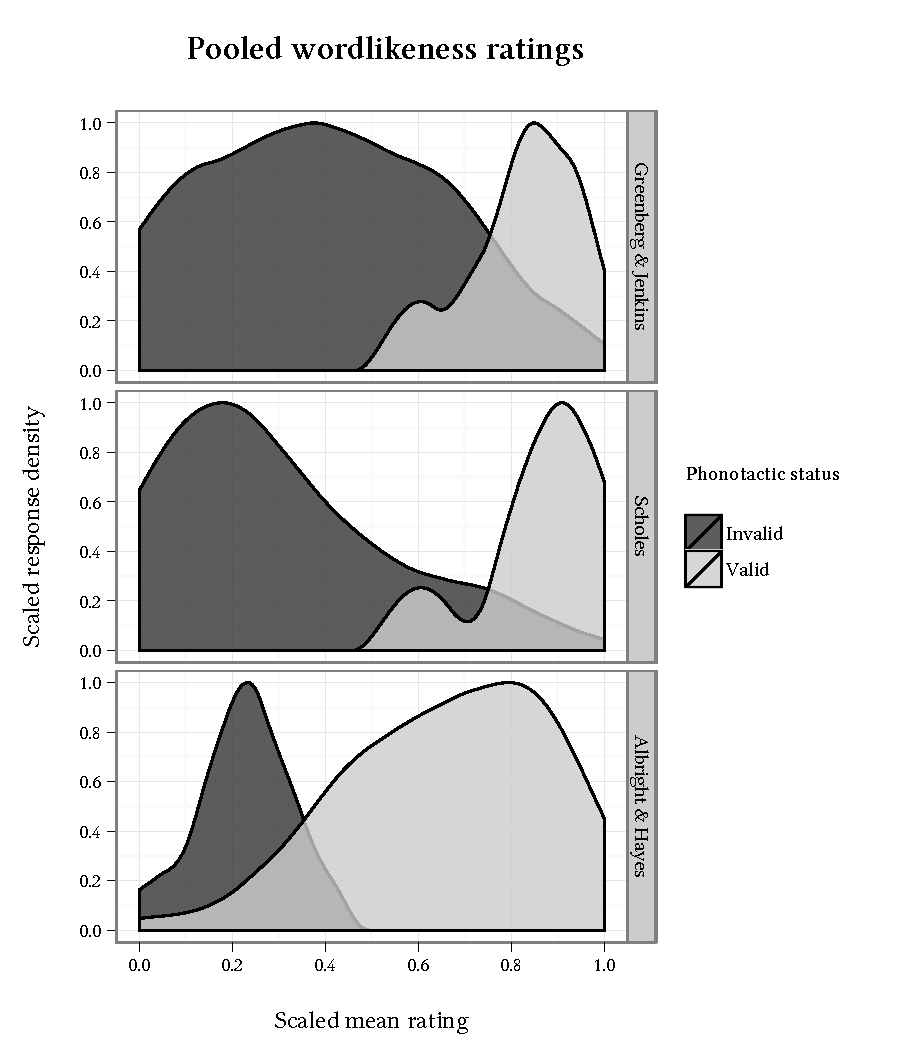
\includegraphics{density.pdf}
\caption{Density of responses}
\label{density}
\end{figure}

\begin{example}
EM test results:

\vspace{0.5\baselineskip}
\begin{tabular}{l | r r | r r r r r r | r r}
\toprule
     & \multicolumn{2}{c|}{one $\mathcal{N}$} & \multicolumn{6}{c|}{mixture of two $\mathcal{N}$s} & \multicolumn{2}{c}{log $\mathcal{L}$ test} \\
     & $\mu$ & $\sigma$ & $\mu_1$ & $\sigma_1$ & mix$_1$ & $\mu_2$ & $\sigma_2$ & mix$_2$ & $\Lambda$ & $p$-value  \\
\midrule
G\&J & 0.378 & 0.295    & 0.150   & 0.090      & 0.436     & 0.554   & 0.278    & 0.564     & 5.190    & 0.158   \\
S    & 0.596 & 0.361    & 0.236   & 0.232      & 0.437     & 0.876   & 0.105    & 0.563 & 48.965    & 1.3\e{-10} \\
A\&H & 0.431 & 0.266    & 0.301   & 0.200      & 0.559     & 0.595   & 0.246    & 0.411 & 16.186    & 0.001      \\
\bottomrule
\end{tabular}
\end{example}

%\ex Residualized correlations
%\begin{tabular}
%\toprule
%ASDF
%\midrule
%G\&J & 
%S    & 
%A\&H & 
%\bottomrule
%\xe

\subsubsection{Prediction distributions}

\begin{table}
\centering

\begin{tabular}{l l l l l}
\toprule
Spearman $\rho$             & MaxEnt         & density        & bigram         & attested onsets/rimes \\
\midrule
\citeauthor{Greenberg1964a} & 0.765          & 0.648          & 0.863          & \textbf{0.845}        \\
\citeauthor{Scholes1966}    & 0.762          & 0.718          & \textbf{0.827} & 0.791                 \\
\citeauthor{Albright2003a}  & 0.429          & \textbf{0.742} & 0.708          & 0.725                 \\
\citeauthor{Albright2007}   & \textbf{0.926} & 0.619          & 0.523          & 0.793                 \\
\bottomrule
Kendall $\tau_b$            & MaxEnt         & density & bigram & attested onsets/rimes \
\midrule
\citeauthor{Greenberg1964a} & 0.585          & 0.462   & 0.692  & \textbf{0.716}      \\
\citeauthor{Scholes1966}    & 0.597          & 0.565   & 0.652  & \textbf{0.664}      \\
\citeauthor{Albright2003a}  & 0.343          & 0.556   & 0.506  & \textbf{0.599}      \\
\citeauthor{Albright2007}   & \textbf{0.788} & 0.462   & 0.371  & 0.659               \\
\bottomrule
Goodman-Kruskal $\gamma$    & MaxEnt & density & bigram & attested onsets/rimes
\midrule
\citeauthor{Greenberg1964a} & 0.684  & 0.462   & 0.692  & \textbf{1.000} \\
\citeauthor{Scholes1966}    & 0.634  & 0.614   & 0.667  & \textbf{0.995} \\
\citeauthor{Albright2003a}  & 0.656  & 0.575   & 0.509  & \textbf{0.953} \\
\citeauthor{Albright2007}   & 0.871  & 0.498   & 0.373  & \textbf{0.977} \\
\bottomrule
\end{tabular}

\caption{Here is my caption.  All values are significant at $\alpha = 0.05$}
\end{table}


\begin{table}
\centering

\begin{tabular}{l r r r}
\toprule
Spearman $\rho$             & MaxEnt              & density             & bigram              \\
\midrule
\citeauthor{Greenberg1964a} & 0.185               & 0.154               & \textbf{0.319}      \\
\citeauthor{Scholes1966}    & 0.122               & 0.174               & \ul{\textbf{0.292}} \\
\citeauthor{Albright2003a}  & 0.011               & \ul{\textbf{0.246}} & 0.203               \\
\citeauthor{Albright2007}   & \ul{\textbf{0.440}} & \ul{0.340}          & 0.016               \\ 
\bottomrule
Kendall $\tau_b$            & MaxEnt              & density             & bigram \\
\midrule
\citeauthor{Greenberg1964a} & 0.135               & 0.077               & \textbf{0.205}      \\
\citeauthor{Scholes1966}    & 0.098               & 0.124               & \ul{\textbf{0.206}} \\
\citeauthor{Albright2003a}  & 0.005               & \ul{\textbf{0.157}} & 0.126               \\
\citeauthor{Albright2007}   & \ul{\textbf{0.340}} & 0.215               & $-$0.017            \\
\bottomrule
Goodman-Kruskal $\gamma$    & MaxEnt              & density             & bigram \\
\midrule
\citeauthor{Greenberg1964a} & \ul{0.158}          & 0.077               & \ul{\textbf{0.205}} \\
\citeauthor{Scholes1966}    & 0.105               & 0.137               & \ul{\textbf{0.214}} \\
\citeauthor{Albright2003a}  & 0.010               & \ul{\textbf{0.162}} & \ul{0.127}          \\
\citeauthor{Albright2007}   & \ul{\textbf{0.376}} & 0.232               & 0.017               \\
\bottomrule
\end{tabular}

\caption{Here is my caption; underlined values are significant at $\alpha = 0.05$}
\end{table}

%\citet{Coltheart1977}
%
%\citet{Hayes2008a}
%\citet{Albright2009a}

% stats thereof
%\citet{Schilling2002}
%\citet{Helguerro1904}
%\citet{Cohen1956}

% EM
\citet{EM}

\footnote{In performing this evaluation, I have benefitted greatly from course notes by Mark Liberman and Stephen Isard.}
%available at \url{http://www.ling.upenn.edu/courses/cogs501/K-meansHW.html}

% -2 log like ratio test

where the difference in degrees o freedom equals $D$

%\ex $\displaystyle \textrm{Reject } H_0 \textrm{ iff } 
%\ex $\displaystyle \Lambda = -2 \textrm{ ln } L_0 + 2 \textrm{ ln } L_1}$ \xe
% > χ^2_{d.f.=D}$ \xe
